

% This is a small sample LaTeX input file (Version of 10 April 1994)
%
% Use this file as a model for making your own LaTeX input file.
% Everything to the right of a  %  is a remark to you and is ignored by LaTeX.

% The Local Guide tells how to run LaTeX.

% WARNING!  Do not type any of the following 10 characters except as directed:
%                &   $   #   %   _   {   }   ^   ~   \

%%%%%%%%%%%%%%%%%%%%%%% file typeinst.tex %%%%%%%%%%%%%%%%%%%%%%%%%
%
% This is the LaTeX source for the instructions to authors using
% the LaTeX document class 'llncs.cls' for contributions to
% the Lecture Notes in Computer Sciences series.
% http://www.springer.com/lncs       Springer Heidelberg 2006/05/04
%
% It may be used as a template for your own input - copy it
% to a new file with a new name and use it as the basis
% for your article.
%
% NB: the document class 'llncs' has its own and detailed documentation, see
% ftp://ftp.springer.de/data/pubftp/pub/tex/latex/llncs/latex2e/llncsdoc.pdf
%
%%%%%%%%%%%%%%%%%%%%%%%%%%%%%%%%%%%%%%%%%%%%%%%%%%%%%%%%%%%%%%%%%%%

\documentclass[conference]{IEEEtran}

%% INFOCOM 2011 addition:
\makeatletter
\def\ps@headings{%
\def\@oddhead{\mbox{}\scriptsize\rightmark \hfil \thepage}%
\def\@evenhead{\scriptsize\thepage \hfil \leftmark\mbox{}}%
\def\@oddfoot{}%
\def\@evenfoot{}}
\makeatother
\pagestyle{headings}
%\usepackage{latex8}
\usepackage{setspace}
\usepackage{times}
%\usepackage{kbordermatrix}% http://www.hss.caltech.edu/~kcb/LaTeX.shtml
\newcommand{\noindex}{\hspace*{-0.8em}}%
\usepackage{pgf}
\usepackage{tikz}
\usetikzlibrary{arrows,automata}
\usepackage[latin1]{inputenc}
\usetikzlibrary{arrows}
\usepackage{epsfig,xspace}
\usepackage{url}
\usepackage{verbatim}
\usepackage{amsmath}
\usepackage{listings}
\usepackage{verbatim}

\usepackage{graphicx}
\usepackage{epstopdf}
\usepackage{mathtools}
%\usepackage{fix2col}
\usepackage{multirow}
\usepackage{varwidth}
\usepackage{algorithm}
\usepackage{algorithm}
\usepackage{algpseudocode}
%\usepackage[dvips]{graphicx}
%\usepackage{mss}
%\usepackage{subfigure}
\usepackage{subfigure}
%\usepackage{nopageno}
%\usepackage{fix2col}

\IEEEoverridecommandlockouts
\lstset{
  basicstyle=\footnotesize,
  columns=flexible,
  morecomment=[s]{/*}{*/}}

\newtheorem{Theorem}{Theorem}[section]
\newtheorem{lemma}[Theorem]{Lemma}
\newtheorem{proposition}[Theorem]{Proposition}
\newtheorem{corollary}[Theorem]{Corollary}

\newcommand{\remove}[1]{ }
\newcommand{\eg}{\emph{e.g.}}
\newcommand{\ie}{\emph{i.e.}}

\newenvironment{proof}[1][Proof:]{\begin{trivlist}
\item[\hskip \labelsep {\bfseries #1}]}{\end{trivlist}}


\newenvironment{definition}[1][Definition]{\begin{trivlist}
\item[\hskip \labelsep {\bfseries #1}]}{\end{trivlist}}
\newenvironment{example}[1][Example]{\begin{trivlist}
\item[\hskip \labelsep {\bfseries #1}]}{\end{trivlist}}
\newenvironment{remark}[1][Remark]{\begin{trivlist}
\item[\hskip \labelsep {\bfseries #1}]}{\end{trivlist}}

\renewcommand{\algorithmicrequire}{\textbf{Input:}}
\renewcommand{\algorithmicensure}{\textbf{Output:}}

\newcommand{\qed}{\nobreak \ifvmode \relax \else
      \ifdim\lastskip<1.5em \hskip-\lastskip
      \hskip1.5em plus0em minus0.5em \fi \nobreak
      \vrule height0.6em width0.5em depth0.0em\fi}

\def\sqzhuge{\vspace{-14pt}}
\def\sqzsec{\vspace{-10pt}}
\def\sqzsmall{\vspace{-8pt}}
\def\sqztiny{\vspace{-4pt}}
\remove{
\usepackage{vmargin}
\setpapersize{USletter}
\setmarginsrb{2.54cm}{2.54cm}{2.54cm}{1.5cm}{0pt}{0mm}{0pt}{8mm}
\setcounter{secnumdepth}{3}
}
\newcommand\Mark[1]{\textsuperscript#1}

\begin{document}
\pagenumbering{gobble}

\title{SSD-Optimized Workload Placement with Real-time Learning in HPC Environments}
\author{\IEEEauthorblockN{Lipeng Wan\IEEEauthorrefmark{1}, Zheng Lu\IEEEauthorrefmark{1}, Qing Cao\IEEEauthorrefmark{1}, Feiyi Wang\IEEEauthorrefmark{2}, Oral Sarp\IEEEauthorrefmark{2}, and Bradley Settlemyer\IEEEauthorrefmark{2}}\\
\vspace{-0.1in}
%\begin{tabular}{*{2}{>{\centering}p{.45\textwidth}}}
\IEEEauthorblockA{\IEEEauthorrefmark{1}Department of Electrical Engineering and Computer Science\\University of Tennessee, Knoxville, TN, US\\
Email: \{lwan1, zhenglu, cao\}@utk.edu} \\
%\vspace{-0.1in}
\IEEEauthorblockA{\IEEEauthorrefmark{2}Oake Ridge National Laboratory\\ Oak Ridge, TN, US\\
Email: \{fwang2, oralhs, settlemyerbw\}@ornl.gov}
%\end{tabular}
\vspace{-0.1in}
}

\vspace{-0.4in}
\maketitle


\vspace{-1in}
\begin{abstract}
In recent years, SSD drives have emerged as a type of viable alternative storage hardware to conventional hard drives (HDD) due to their high speed and decreasing cost. However, the durability of SSD chips are still considerably limited and thus, pure SSD based solutions have not been economically feasible. In this paper, we focus on the problem of workload and storage placement in HPC (High-Performance Computing) environments, and propose
a hybrid solution where SSDs and HDDs are used together as the storage hardware for object placement purposes. Based on an analytical model, we propose an optimized scheme that places workload on storage units provided by SSDs and HDDs in a topology-aware manner so that their performance and lifetime may be optimized. The scheme is also enhanced with an adaptive learning algorithm where real-time classification methods are employed to determine the best placement of objects during runtime. We present preliminary results based on this approach using a simulator we developed to show that the analytic model approach can dynamically adjust storage placement as workloads evolve to enhance performance and lifetime.


\end{abstract}

%\IEEEpeerreviewmaketitle


\section{Introduction}
\label{intro}

Providing resilient and fast storage service for HPC applications remains a critical challenge given the large demands on storage space as well as the possibility of disk drive failures~\cite{}. Therefore, it is crucial to schedule storage properly among multiple drives based on the nature of workloads as well as the properties of the underlying hardware. On the other hand, both the workloads and the underlying hardware evolve over time, meaning that algorithms have to be designed to take these changes into their consideration.

One particular trend that has emerged in recent years is the use of SSD drives in storage to provide \emph{premium} services, as the reading and writing speed for SSD drives are typically faster compared to the hard drives~\cite{}. On the other hand, SSD drives also have different failure patterns as repeated reading and writing of the same blocks will cause the drives to fail. Furthermore, SSD drives are also limited in capacity, meaning that they can only serve as a cache, rather than replacements, for conventional hard disks. Therefore, how to integrate SSD drives successfully into the design of a storage area network becomes a challenge that modern HPC applications have to handle.

Existing algorithms to integrate SSD drives can already be found in the literature~\cite{}. These methods, while effective, suffer from three drawbacks. First, they are largely based on heuristic algorithm designs that are either developed in isolation with the runtime workload, or are based on static assumptions on the workload patterns, making them unsuitable when the underlying workloads and demands change over time. Second, they do not properly handle user demands, where specific requirements on the data storage placement may exist. Finally, they do not consider drive failures, which has considerable impact when underlying hardware becomes unavailable.

To address these problems, we present a holistic approach where we aim to develop a framework that adaptively classifies workloads, adjusts the placement of storage objects, and fulfills the needs of the users with regard to their storage requirements. By adaptive, we mean that the developed algorithm can self-tune to the underlying hardware and software environments. Our developed algorithm has the following assumptions. First, we consider that the storage hardware consists of both conventional hard drives and SSD drives. SSD drives are typically smaller in capacity, but faster in terms of speed. Hard drives and SSD drives have different parameters for failures. Second, the user may request changes to the placement of replications for data, as well as the number of replications, over the workload lifetime. We assume such changes could come in a high rate, leading to rapid replacement changes to be generated. Therefore, it is necessary that our modeling algorithms keep up-to-date predictions on the objects' future access rates so that they can rebalance such object storage in real time.

Specifically, the proposed framework contains two major novel contributions: machine learning based workload classification and demand-aware object placements. In both parts, we present novel algorithms and evaluate their performance. We next describe these two contributions separately.

In the first contribution, our key idea is to classify data objects and their access patterns based on a fusion of multiple information sources including the history of data accesses and the workloads that access them in the past. Based on such information, we determine those objects that are most likely to be frequently accessed in the future, and we move them to the SSD-powered drives so that their access latency can be minimized, under the constraint that the moving cost will be offset by the access latency savings. The detailed classification model for the objects can be flexible: our preliminary study classifies each data object during runtime based on a Markov chain model that is enhanced by machine learning techniques. Specifically, our goal is to predict whether this data object will be accessed frequently in the future. Once such predictions are made, they will be used as improvements to the existing algorithms such as the CRUSH algorithm that has been widely used for data storage placement in high performance computing platforms.

In the second contribution, we take into account the underlying network topology and bandwidth in our modeling, so that we can periodically recalculate the object deployment when something changes. To this end, we also take into account the user requirements, such as their preferences on where to place the objects, and the underlying topology relations. For example, if the user specifies that no two copies of the same storage object should be on the same rack, such a requirement should be fulfilled properly by the storage algorithm.

%The key contributions of the developed algorithm are listed as follows: first, we present an access-frequency sensitive algorithm for extending the CRUSH algorithm. The core methodology involves modeling the different storage services based on their access latency parameters, and try to minimize the overall access time through an optimization problem.
%
%Second, we observe that given that users' request patterns change over time, it is time-consuming to re-solve the problem every time the user input changes. Therefore, we develop a learning algorithm to classify the input patterns, and generate the output parameters automatically after the training phase. This approach allows the extension of CRUSH to handle different application requirements highly efficiently.


The rest of this paper is organized as follows. We describe the related work in Section~\ref{sec:relatedwork}. The design is described in Section~\ref{sec:design}.   The performance evaluation is given in Section~\ref{sec:evaluation}. The application case study is given in Section~\ref{sec:application}. We provide conclusions in Section~\ref{sec:conclusion}. %We survey related work in Section~\ref{sec:related}.

















\section{Related Work}
\label{sec:relatedwork}

In this section, we provide a brief introduction on several existing works
which are related to our paper. We classify these existing works into two
categories. The first category consists of existing works on data placement
algorithms for distributed storage systems, while the second consists of those
on hybrid storage systems which aim to leverage SSD drives to improve data
access performance.

As large-scale distributed storage systems have been extensively used in HPC
area, the problem of distributing several petabytes of data among hundreds or
thousands of storage devices becomes more and more critical. To address this
problem, many data placement algorithms have been proposed. For instance,
Distributed Hash Tables (DHTs) have been used to place and locate data objects
in P2P systems \cite{Stoica2001, Ratnasamy2001, Cai2004}. Another replica
placement scheme called chain placement was also proposed and applied to some
P2P and LAN storage systems \cite{Rowstron2001, Lee1996, MacCormick2004}.
Honicky and Miller presented a family of algorithms named RUSH
\cite{honicky04} which utilizes a mapping function to evenly map replicated
objects to a scalable collection of storage devices and meanwhile supports the
efficient addition and removal of weighted devices.

To resolve the reliability and replication issues RUSH algorithms suffered in
practice usage, Weil et al. proposed a scalable pseudo-random data
distribution algorithm named CRUSH \cite{Weil2006} upon which our algorithm is
based. Besides optimally distributing data to available resources and
efficiently reorganizing data after adding or removing storage devices, CRUSH
exploits flexible constrains on replica placement to maximize the data safety
in the situation of hardware failures. CRUSH algorithm allows the
administrator to assign different weights to storage devices so that
administrator can control the relative amount of data each device is
responsible for storing. However, the device weights used in CRUSH algorithm
only reflect the capacities of storage devices, which means CRUSH algorithm
might not be effective anymore for hybrid storage systems consists of both SSD
and HDD devices since these two kinds of storage devices have totally
different performance characteristics.

Existing works on hybrid storage systems usually concentrate on two major
directions: either using a small amount of SSD-based storage as a cache
between main memory and hard disk drives or integrating SSD and HDD together
to form a hybrid storage system. Because of SSD devices' high cost and small
capacity, the cache-based solution is understandable and common. For example,
Srinivasan et al. designed a block-level cache named Flashcache
\cite{Flashcache} between DRAM and hard disks using SSD devices. Zhang et al.
proposed iTransformer \cite{Zhang2012} which exploits a small SSD to schedule
requests for the data on disks so that high disk efficiency can be achieved.
SieveStore \cite{Pritchett2010} adopts a selective caching approach in which
the access count of each block is tracked and the most popular block is cached
in SSD device.

Recently, efforts have been made to combine SSD and HDD together to construct
a hybrid storage system in which SSD is used as a storage device same as HDD
rather than a cache. Chen et al. designed and implemented a high performance
hybrid storage system named Hystor \cite{Chen2011}, which identifies data
blocks that either can result in long latencies or are semantically critical
on hard disks and store them in SSDs for future accesses. In order to reduce
random write traffic to SSD, Ren et al. proposed I\_CASH \cite{Yang2011} which
exploits the spacial locality of data access and only store seldom-changed
reference data blocks on SSD. Besides, ComboDrive \cite{Payer2009}
concatenates SSD and HDD into one address space via a hardware-based solution
so that certain data on HDD can be moved into the faster SSD space.

There are two main differences between existing works on hybrid storage
systems and our approach: First, most existing works on hybrid storage systems
only consider how to improve the utilization of SSD devices while they ignore
the reliability and replication issues that data placement algorithms, such as
CRUSH, try to resolve in HPC environment; Second, our approach tries to
monitor the usage of data blocks and store performance critical data on SSD
devices which is kind of similar to several existing works, like
\cite{Chen2011, Luo2012}, but beyond this, our approach applies machine
learning algorithm to predict the future usage of data blocks and store
potential critical data on SSD in advance.

\section{Algorithm Design}
\label{sec:design}

In this section, we introduce the design of the algorithm. We first present the problem formulation. Then, we present an overview of its structure. Finally we present a detailed description of its components and related algorithms.


\subsection{The Problem Formulation}
\label{problemformulation}

The key problem we are considering for the storage provisioning is to develop a sufficient, yet not wasteful, set of storage allocations from existing hardware for objects to be stored, so that applications can meet their desired performance. This problem of storage allocation is challenging due to: (1) the dynamics of workload, (2) the requirement of users, e.g., no replicas should be stored on the same rack for reliability, etc. and 3) difficulty and overhead of deriving the storage allocation results for each workload and user requirement combination. As
a result, it is difficult to determine the storage allocation that will
achieve the desired quality of service while minimizing the hardware cost and storage overhead. Therefore, if we model such a problem as a search problem whose solution is from a very large search space, then it is very hard to always reach the optimal configuration when something changes, even such change could be slight.
%
%In most cases we can resort to offline algorithms, where the results are calculated and used for a rather long period of time in storage services. This of course leads to underwhelming performance and storage waste. The key issue with existing solutions is that they do not handle dynamics in the requests or workloads successfully. Moreover, on-line algorithms may not be fully predictable in their convergence time, leading to long delays and out-of-date solutions. This problem may become even worse when different types of hardware such as SSD is used, or servers may be added or removed due to failures, and so on.

Based on such concerns, we formulate the following problem: \textbf{given the underlying demands, how can we find an optimized storage placement that can incrementally provide results that can achieve the best performance under the resource constraints and user requirements?} Note that given that the users' request may change frequently, we would like to be able to re-use previous calculation results as much as possible, so that we can avoid the re-calculation when a similar scenario is met in practice.

\begin{figure}[t]
\begin{centering}
  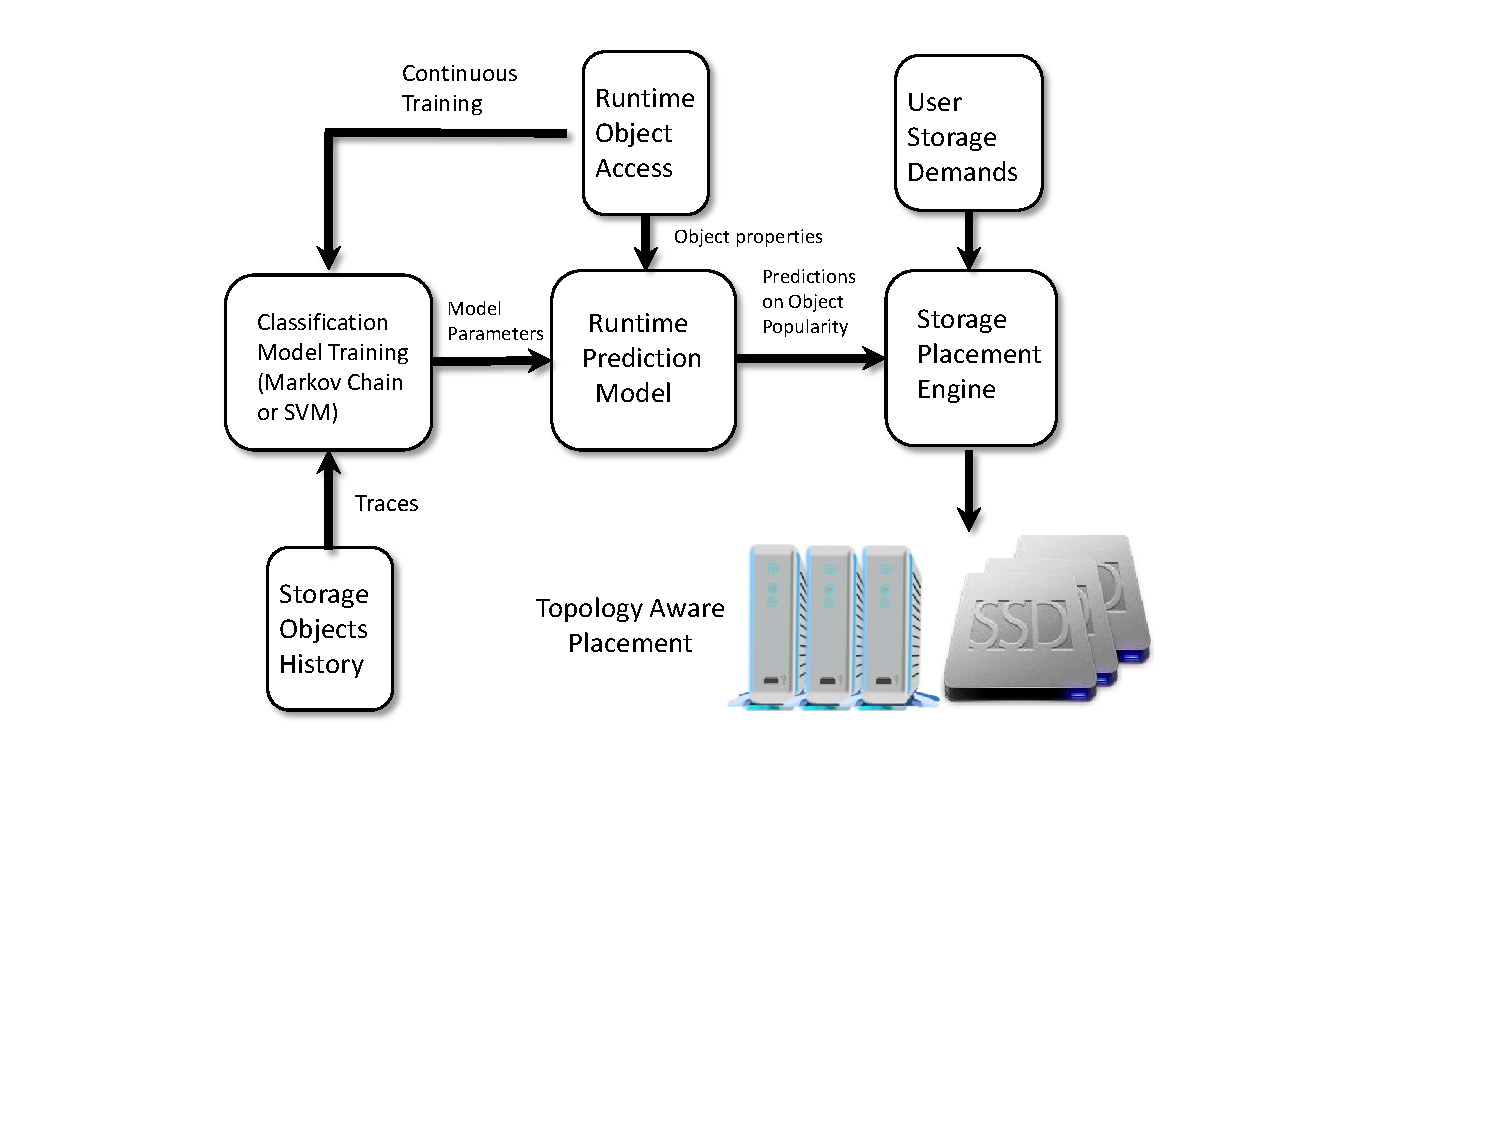
\includegraphics[width=3.3in]{./ModelPhase.pdf}
  \caption{The architecture of workflow}\label{fig:architecture}
  \label{arch}
\end{centering}
\vspace{-0.1in}
\end{figure}


\subsection{Architecture Overview}
\label{architecture}

Figure~\ref{arch} shows the overall architecture of the proposed workflow, where the whole procedure works as follows:  the first core component, the classification model, is trained based on the access history of storage objects. It then provides the model parameters for the runtime prediction model, which is used to classify runtime access to objects. Such accesses are classified into either ``recurring'' or ``non-recurring'', depending on whether the objects are considered to be popular or not. The popularity metric for objects, as well as the user storage demands, are then handled by the storage placement engine to move storage objects as needed. Note that such placement of data can be either on the hard disks or SSDs, depending on users' requirements. Finally, the runtime object access traces are also used as input for the classification model for continuous training purposes.


\subsection{Design Assumptions}

We now present our design assumptions. We assume that the user of the service deploys their service across a pool of storage servers. The storage servers could be a set of OSDs, which are intelligent controllers that can map the requests from the user to the storage services. Each of the OSD may provide some level of SLO (Service Level Objective) for the deployed service.

During the system's operation, we assume that users' requests include both reading and writing operations. Note that the writing operations may be dominating for certain workflows, such as checkpoint backups that require periodic operations~\cite{}. The users' workloads may also change over time, which requires that the system should adapt to the requirements and demands.



\subsection{Learning based Workload Classification}

In this section, we describe how the classification model generates model parameters based on storage object history traces. Specifically, once the features are selected, we then collect training data for a period of time. The task then becomes a classification problem, where we need to evaluate the effect of selected features on classification accuracy. In our design, we adopt a Markov chain based approach. More specifically, suppose that we select $N$-tuple that forms a workload signature as:

\[
  Signature = {m^1, m^2, ..., m^n}
\]

where the $m_i$ represents a measured metric of $i$. Note that the metric selection process is fully automated and transparent to the user.

Once the signatures are collected, it is important that we can classify later workloads based on the training periods. This is based on the assumption that user workloads will have inherent repeating patterns, where similar workloads may be encountered again. This therefore resembles the ``cache hit rates'' which are well studied in the computer cache designs. But still there are considerable differences, as unlike cache contents, the workload signatures may indeed shift over time. Therefore, it is only giving approximate solutions, not accurate answers.

Note that there is a tradeoff in the overhead of training and prediction and the achieved hit rates. We need to achieve a good tradeoff in this design. We make the following assumptions regarding OSDs. First, we assume that each OSD can maintain the access history for each data object. In reality, it may not be practical to record a long access history for each data object since in that case the storage overhead could be huge, instead, only recent access history are maintained and updated periodically. Second, we model the access frequency of each data object using a discrete-time Markov chain in which each state represents a specific range of access frequency. With the access history, we can estimate the parameters of the Markov chain model. Third, by calculating the stationary distribution of the Markov chain, we can predict how possible the access frequency of each data object lies within certain range in the long run. Finally, we rank each data object based on the weighted sum of the stationary distribution and the weights are chosen according to the specific range represented by each state in the Markov chain. The highest rank the data object has, the more possible it will be moved to SSD devices.

\subsubsection{Access History of Data Objects Collection}

Fig. \ref{trace} demonstrates the access frequency (Here the ``access'' includes both reads and writes.) of a data object during one month.  The x axis of Fig. \ref{trace} is the range of one month time which has been divided into 720 sections (each section is 1 hour) and each point on x axis represents each of these time sections. The y axis represents the number of times the data object has been accessed during each time section.

\begin{figure}[!t]
\centering
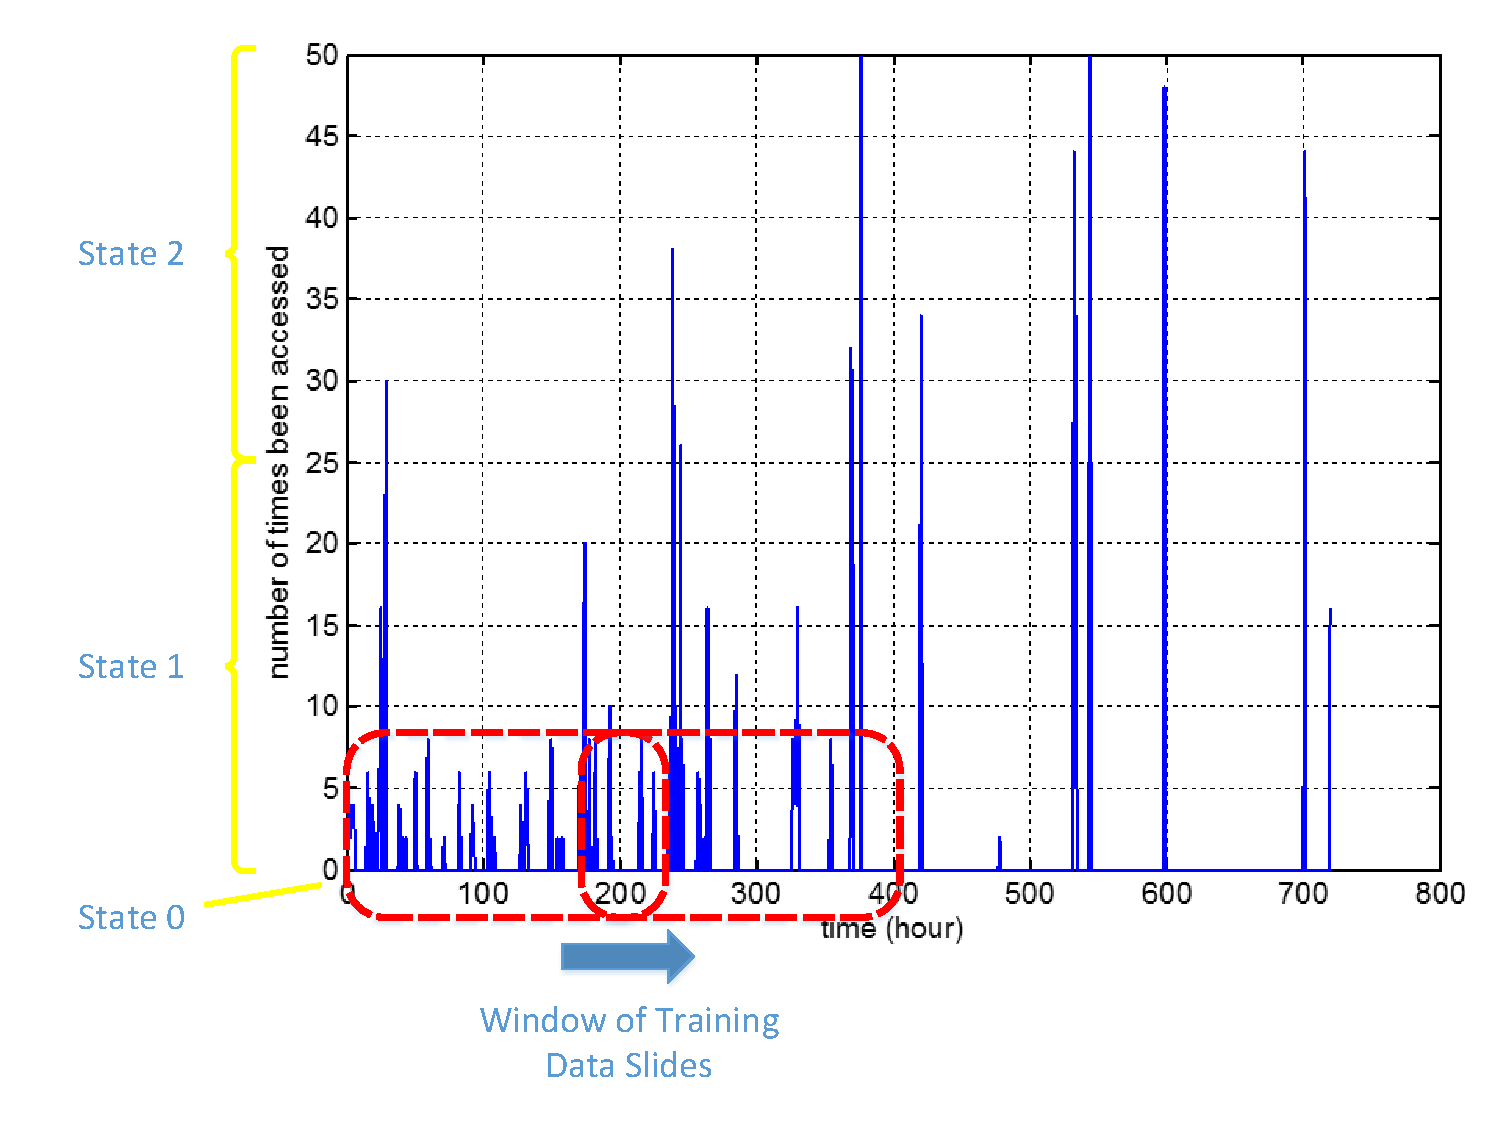
\includegraphics[width=3.0in]{./trace.pdf}
% where an .eps filename suffix will be assumed under latex,
% and a .pdf suffix will be assumed for pdflatex; or what has been declared
% via \DeclareGraphicsExtensions.
\caption{Trace of Data Object Access Frequency}
\vspace{-0.25in}
\label{trace}
\end{figure}

As we mentioned at the beginning of this section, since the storage overhead, maintaining the entire access history of each data object on each OSD is not acceptable. Thus, we only maintain recent access history of each data object and use such access history to build a Markov chain model to predict the future access frequency. As shown in Fig. \ref{trace}, only the access history in the window which has red dot borderline is used to train the prediction model and the window of training data slides with time so that we can implement online prediction for data objects access frequency.

\subsubsection{Markov Chain Predication Model}

With the access history of each data object, we can now build the Markov chain model to predict the future access frequency of data objects. First, we need to determine how many states the Markov chain should have and the range of access frequency each state represents. For example, as shown in Fig. \ref{trace}, if the maximum number of access times during an observation period is 50, then we can divide 50 evenly and build a Markov chain model that has 3 states. If during a time section, there is no access of the data object, then the Markov chain will stay in state 0. If during a time section, the number of access times is larger than 0 but less than 25, then the Markov chain will stay in state 1, and so on. The transition diagram of the Markov chain is shown in Fig. \ref{transitioin}.

\begin{figure}[!t]
\centering
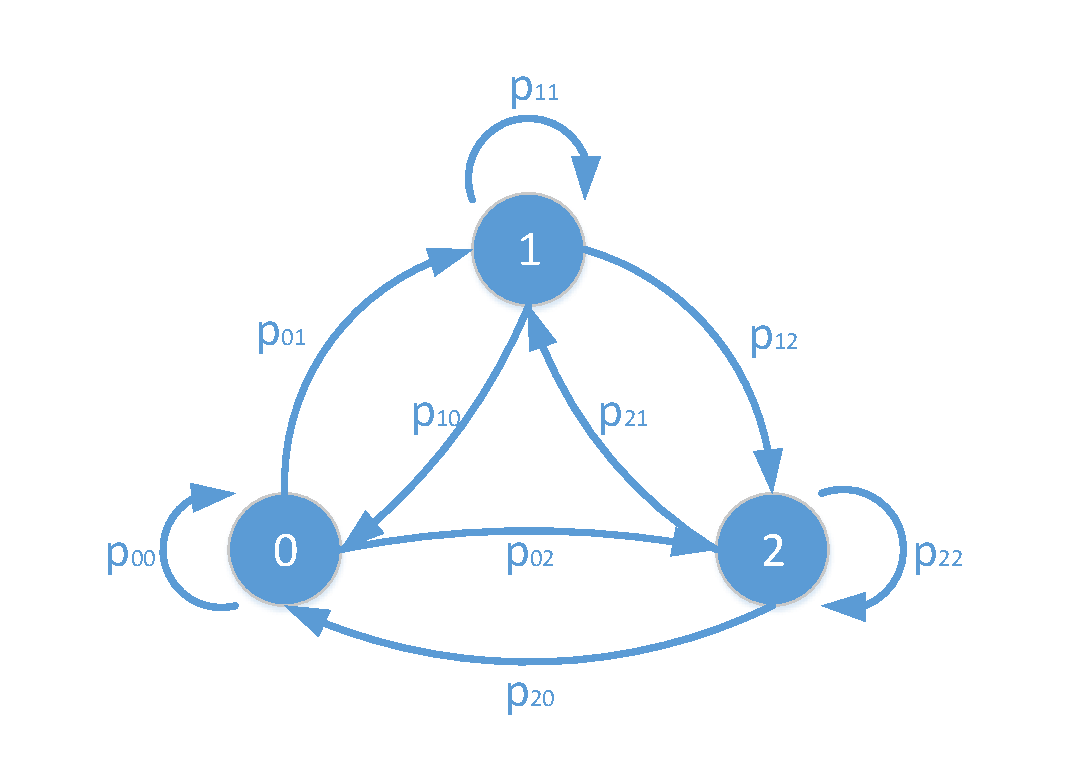
\includegraphics[width=3.0in]{./transition.pdf}
% where an .eps filename suffix will be assumed under latex,
% and a .pdf suffix will be assumed for pdflatex; or what has been declared
% via \DeclareGraphicsExtensions.
\caption{Transition Diagram of Markov Chain}
\vspace{-0.25in}
\label{transitioin}
\end{figure}

Second, we transform the access history to the state transition sequence of the Markov chain based on the specific range each state represents. For example, after transformation the state transition sequence of access history shown in Fig. \ref{trace} is: 1,1,1,1,1,0,0,... Based on the state transition sequence, we can estimate the transition probabilities between every two states and construct the transition matrix of the Markov chain shown below:
\begin{equation}
\mathbf{T} =
 \begin{pmatrix}
  p_{00} & p_{01} & p_{02} \\
  p_{10} & p_{11} & p_{12} \\
  p_{20} & p_{21} & p_{22}
 \end{pmatrix}
\end{equation}

According to the properties of Markov chain, we have:
\begin{equation}
\lim_{n\to\infty}\mathbf{T}^{n} =
 \begin{pmatrix}
  \pi_{0} & \pi_{1} & \pi_{2} \\
  \pi_{0} & \pi_{1} & \pi_{2} \\
  \pi_{0} & \pi_{1} & \pi_{2}
 \end{pmatrix}
\end{equation}
in which $\boldsymbol{\pi} = [\pi_{0}, \pi_{1},  \pi_{2}]$ is called the stationary distribution of the Markov chain. We can simply calculate $\boldsymbol{\pi} $ through computing a normalized multiple of a left eigenvector $\mathbf{e}$ of the transition matrix $\mathbf{T}$ with an eigenvalue of 1:
\begin{equation}
\boldsymbol{\pi} = \frac{\mathbf{e}}{\sum_{i}e_{i}}
\end{equation}
Since the stationary distribution $\boldsymbol{\pi}$ reflects the probabilities that each state of Markov chain will be visited in the future, which can be used to predict the access frequency of each data object.

Finally, we need to rank the data objects on an OSD based on the prediction results so that we can determine which data object should be moved to SSD devices. As different states of the Markov chain represent different access frequency ranges, they have different importance to the prediction results. For example, even if the calculated stationary distribution tells us state 1 will be visited with higher probability than state 2, to rank the importance of the data object, we must consider that state 2 represents higher access frequency. Therefore, we use a weighted sum of the stationary distribution to rank the importance of the data object and the weights are defined by values that are proportional to the access frequency ranges the states represent. For example, if we obtain the stationary distribution of the data object is $\boldsymbol{\pi} = [0.31, 0.56, 0.13]$, and we assign weights $[0, 10, 20]$ to the three different states, we can calculate the rank of the data object by $rank_{obj_{x}} = 0.31\times0+0.56\times10+0.13\times20 = 8.2$.

\subsection{Parametric User Demand Profiling}

The second novel contribution of our work is that we will adapt the storage placement based on user demands, such as the locations of redundant copies and the frequency of making duplicates, in the face of possible failures. In this aspect, we assume that users' requests will be parametric, meaning that all requests will be embedded into equations or constraints. For example, a requirement on the number of redundant copies can be expressed as $RedundantCopy > 3$.  Therefore, for the storage placement algorithm to be effective in dealing with such dynamic requirements, it first needs to receive such demands from users, and their associated storage needs. To profile a requirement, our algorithm uses a profiler that is deployed along the path of the users' requests. The profiler serves requests in the profiling environment, allowing us to collect all metrics that are needed for the characterization of users' requirements. Note that such profiling is occurring independently of the OSD servers that handle such requests concurrently.

The advantage of having the profiler operating independently of the OSDs lies in that this does not require our profiler to be tightly integrated into the rest of the system. Therefore, the profiler can be easily replaced as needed, which gives us additional flexibility.

The central task of the profiler is that it will pick the requirement one by one and fulfill them, depending on their urgency and the amount of resources needed to fulfill them. For the profiling to be most effective, it is critical to pick a set of metrics that form the bottleneck. This is based on the observation that once we fulfill one bottleneck requirement, usually more than one requirements will be met. 
 
Ideally, the collected metrics for the incoming workloads should allow us to uniquely find a placement of storage OSDs without the details of the workloads themselves. This is because the algorithm is by nature greedy, and in the worst case, it will traverse all possible requirements from the user and fulfill them. 

%\section{Analytical Modeling of Algorithm Performance}
\label{analysis}

In this section, we model the system performance using analytic approaches. 

\section{System Evaluation}
\label{evaluation}

\subsection{Evaluation Overview}

In this section, we systematically present the evaluation of the proposed algorithm. We implement the algorithm in both simulations and a testbed on the Amazon EC2 platform. We focus on its performance metrics including the throughput, reading latency, replication ratio, and availability. Details are presented below.

Metrics definitions and goals


\subsection{Setup of Evaluations}

We evaluate the performance of our learning algorithm by replaying realistic workload traces. We use a long-term I/O traces, LASR traces~\cite{}, which are taken at system-call level in 2000 and 2001 as part of a security research project.
We track different files' access time during their lifetime. We divide the time into fixed length time slots and count how many times each file has been accessed during each time slot.
Through all the files that have been accessed in a trace, we select 1700 files of them which are more frequently accessed and study their access frequency and time relation.
By analyzing the access of these frequently accessed files, we find out that most of these files can be put into two categories according to the access patterns during their lifetime.
The first category is files which has constant access patterns. Files in this category have been frequently accessed during their whole lifetime, without too much difference between the maximum access point and minimum access point.
Fig. 1 shows a typical file falls into this category. The learning algorithm, especially the Markov chain approach can achieve a higher level of accuracy for this kind of files.
The second category is files with a burst access pattern. Files in this category have only been accessed at very few time slots, but the access count for each time slot that has been accessed is very large.
Fig. 2 shows a typical file falls into this category. Currently, it is pretty hard for any learning algorithm including Markov chain approach to make a good decision for this kind of files.



\subsection{Evaluation Results}

We plot the results in the following figures.

%\section{Application Case Study}
\label{casestudy}

\subsection{Problem Overview}

Describes the workload problem

\subsection{Details}

Describes the details of the implementation for this application case study. 
\section{Conclusions}
\label{conclusion}

 

{\small
\nocite{*}
\bibliographystyle{IEEEtran}
\bibliography{reference}
}

\end{document}
